\chapter{Resultados e Discussão}\label{cap:resultados}

\section{Desafio em trajeto especifíco fácil}

O primeiro e único treino foi executado como agente percorrendo somente um percurso em linha reta, conforme a imagem abaixo.

\subsection*{Resumo}

O treino foi no \textit{path(8)} da estrutura do projeto (ver apêndice).
% TODO: criar um apêndice  da estrutura completa de gameobjects do projeto
\begin{table}[htpb]
    \centering
    \caption{Configuração do treino do trajeto específico fácil}
    \begin{tabular}{|l|p{2cm}|p{3cm}|p{3cm}|p{3.5cm}|}
         \hline
         \small{Rota(s)} & \small{Algoritmo} &          \small{params. PPO}         & \small{params. gerais} &          \small{params. RN}        \\ \hline
            Path(8)      &      PPO          &     beta: 1e-5 \newline epsilon: 0.3 &    max\_steps: 5e5  &    num\_layer:2 \newline hidden\_units:128  \\ \hline
    \end{tabular}
 \end{table}

\begin{figure}[h]
    \centering
    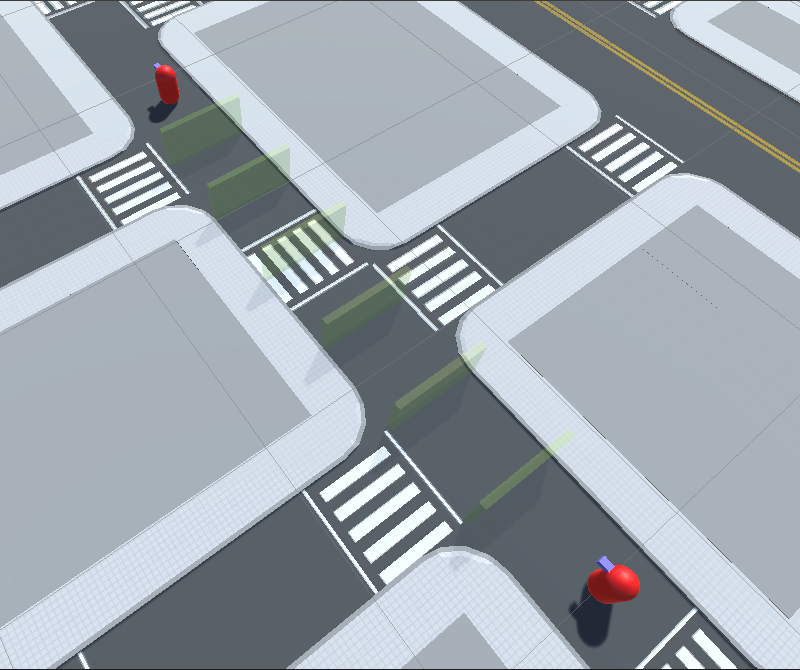
\includegraphics[scale=0.35]{figs/rotas/path_14.png}
     \caption{O percurso executado no primeiro treino. A cápsula vermelha no canto inferior direito indica a posição inicial do veículo e a na parte superior esquerdo indica o destino.}
     \label{fig:rota-1}
\end{figure}
 
\subsection*{Estatísticas}

Abaixo segue os gráficos dos dados coletados deste treino. 

\begin{figure}[h]
    \centering
    \includegraphics[scale=0.35]{figs/treinos/treino-1/política.png}
     \caption{Estatísticas referentes a política. O primeiro gráfico é a entropia, decaindo como é esperado. O terceiro gráfico é o Extrinsic Value estimate, sobe e estabiliza, conforme esperado}
     \label{fig:treino-1-politica}
\end{figure}

\begin{figure}[h]
    \centering
    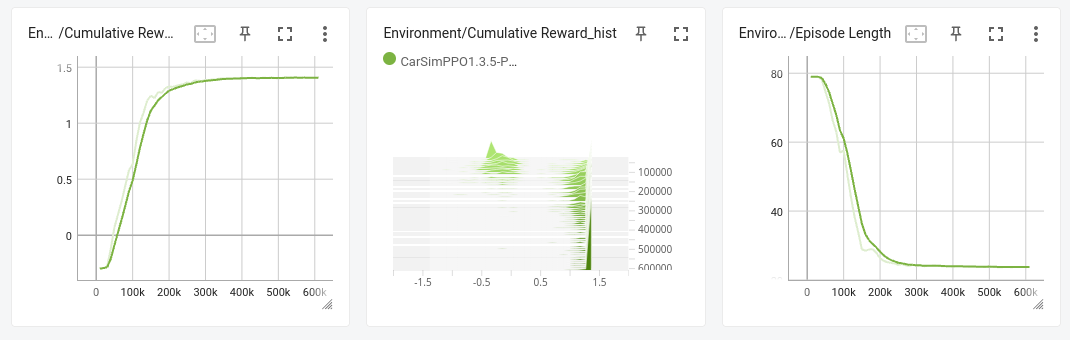
\includegraphics[scale=0.35]{figs/treinos/treino-1/ambiente.png}
     \caption{Estatísticas do ambiente. O primeiro gráfico é o acumulado de }
     \label{fig:treino-1-ambiente}
\end{figure}

\section{Análise}
O treino foi bem sucedido, o agente soube conduzir bem o veículo. Vendo o gráfico 1 da figura 9, pode se notar o crescimento exponencial da recompensa e então sua estabilização quando atinge o máximo da recompensa que é possível receber. Também percebe-se que na mesma velocidade mas desta vez em sentido descendente a duração média do episódio, rapidamente cai pois o agente já dominou o trajeto. Isso é o suficiente para este trajeto, podemos treinar o agente em um novo desafio especifíco mas com um trajeto mais complexo.